\documentclass[compress]{beamer}
\usetheme[darktitle,framenumber]{UniversiteitAntwerpen}

\usepackage[english]{babel}
\usepackage[utf8x]{inputenc}
\usepackage{graphicx}
\usepackage{hyperref}
\usepackage{color}
\usepackage{blkarray}
\usepackage{subfigure}

\title{The power of two paths in grid computing networks}
%\subtitle{This is a dummy subtitle}

\author{Wouter ibens}

\begin{document}
\maketitle

\begin{frame}
\frametitle{Overview}
\tableofcontents
\end{frame}

\section{Setup}
\begin{frame}
\frametitle{Setup}
\begin{figure}[h!tb]
\centering
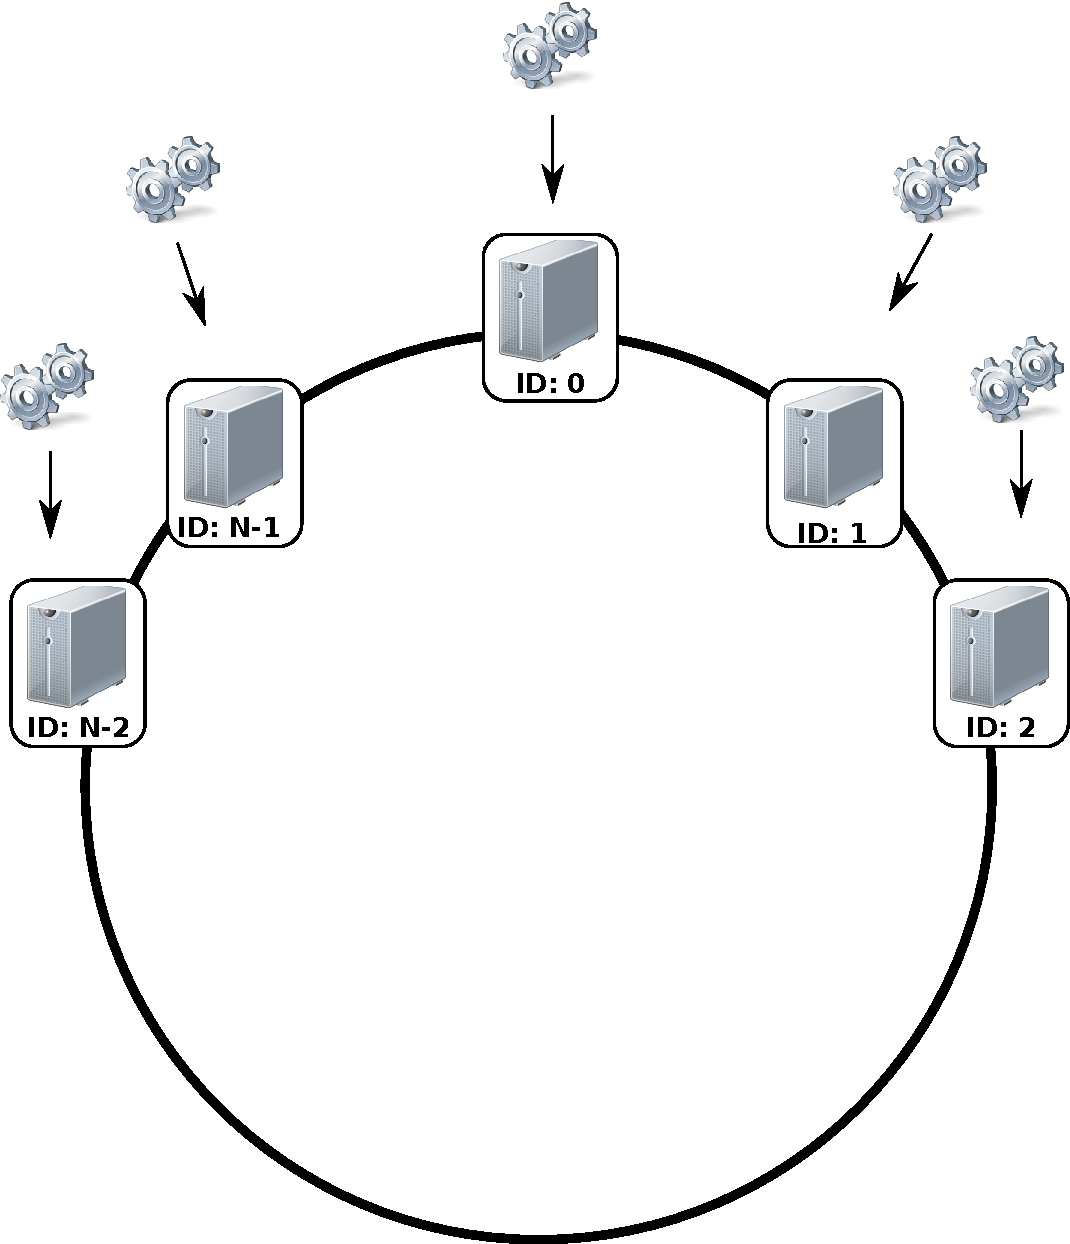
\includegraphics[width=0.7\textwidth,clip=true,trim=0px 225px 0px 0px]{../resources/drawing.pdf}
\end{figure}
\end{frame}

\section{Algorithms}

\begin{frame}
\frametitle{Forward to neighbor - Algorithms}
\begin{itemize}
 \item Forward right \begin{figure}[h!tb]
 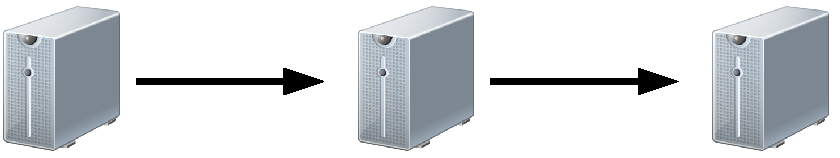
\includegraphics[width=0.7\textwidth]{../resources/p_forwardright.pdf}
 \end{figure}
 \item Left/right forward \begin{figure}[h!tb]
 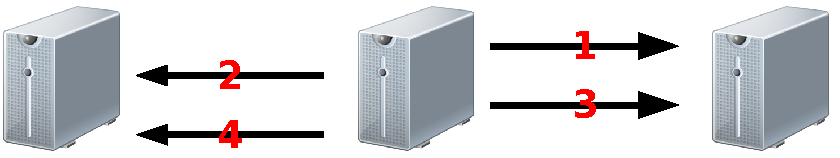
\includegraphics[width=0.7\textwidth]{../resources/p_forwardleftright.pdf}
 \end{figure}
\end{itemize}
\end{frame}

\begin{frame}
\frametitle{Forward to neighbor - Algorithms}
\begin{itemize}
 \item Random left/right with parameter $p$ \begin{figure}[h!tb]
 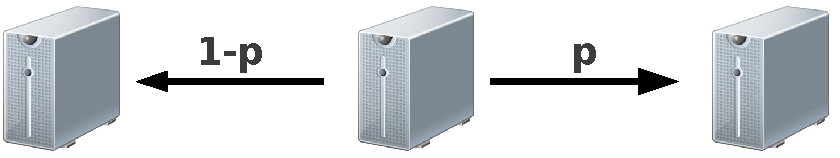
\includegraphics[width=0.7\textwidth]{../resources/p_randforward.pdf}
 \end{figure}
 \item Position dependent \begin{figure}[h!tb]
 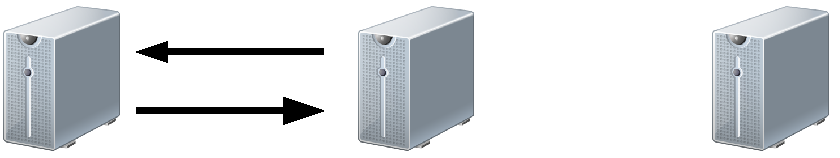
\includegraphics[width=0.7\textwidth]{../resources/p_position.pdf}
 \end{figure}
\end{itemize}
\end{frame}

\begin{frame}
\frametitle{Forward anywhere - Algorithms}
\begin{centering}
Random unvisited
\begin{figure}[h!tb]
 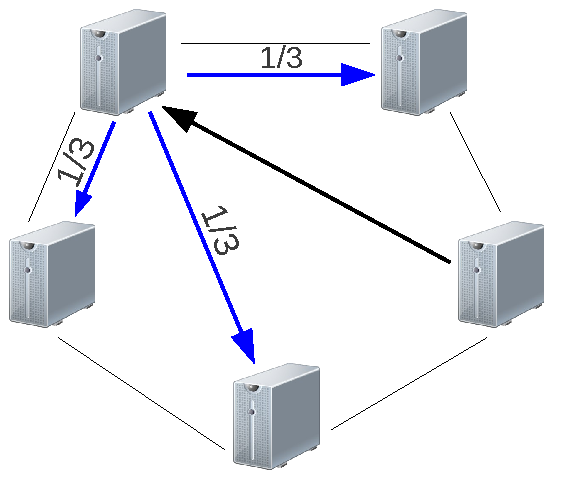
\includegraphics[width=0.7\textwidth]{../resources/p_randunvisited.pdf}
 \end{figure}
\end{centering}
\end{frame}

\begin{frame}
\frametitle{Forward anywhere - Algorithms}
\begin{centering}
(Random) Coprime offset
\begin{columns}
\begin{column}{0.7\textwidth}
\begin{figure}[h!tb]
 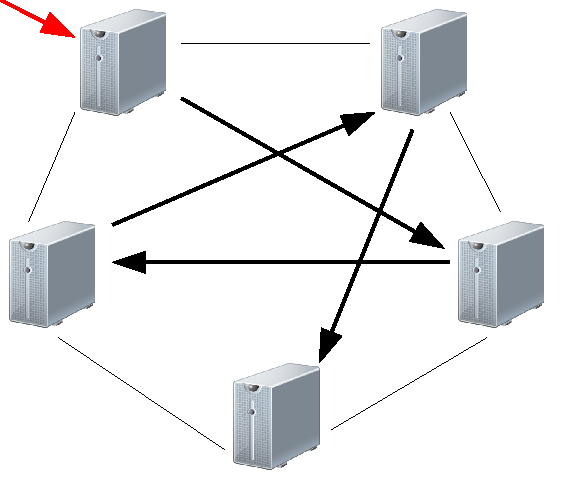
\includegraphics[width=\textwidth]{../resources/p_coprime.pdf}
 \end{figure}
\end{column}
\begin{column}{0.3\textwidth}
N=5 \\
Coprimes:\\
\{1, 2, 3, 4\}

\end{column}
\end{columns}
\end{centering}
\end{frame}

\begin{frame}
\frametitle{Space requirements algorithms}
\begin{table}[h!]
\centering
\begin{tabular}{|p{0.45\textwidth}|p{0.20\textwidth}|p{0.20\textwidth}|} \cline{2-3}
\multicolumn{1}{l|}{}		& Job				& Node \\ \hline
Forward right			& 0				& 0		\\ \hline
Left/right forward		& 1				& 1		\\ \hline
Random left/right forward (p)	& 1				& 0		\\ \hline
Position dependent forward	& 1				& 0		\\ \hline
Random unvisited		& $N-1$				& 0		\\ \hline
Coprime offset			& $\lceil log_2 \varphi(N) \rceil$	& $\lceil log_2 \varphi(N) \rceil$ \\ \hline
Random coprime offset		& $\lceil log_2 \varphi(N) \rceil$	& 0		\\ \hline
\end{tabular}
\end{table}

\[
\varphi(N) ~=~ \sum_{0 < p < N, p \perp N} 1 ~=~  N \cdot \prod_{p|N, p\text{ is prime}} (1-\frac{1}{p})
\]

\end{frame}

\section{Simulation}
\begin{frame}
\frametitle{Simulator}
\begin{itemize}
 \item C++, STL
 \item OpenMP
 \item Source code: \url{http://code.google.com/p/powerofpaths/}
\end{itemize}
\end{frame}

\begin{frame}
\frametitle{Forward to neighbors - Results}
\begin{figure}[h!tb]
 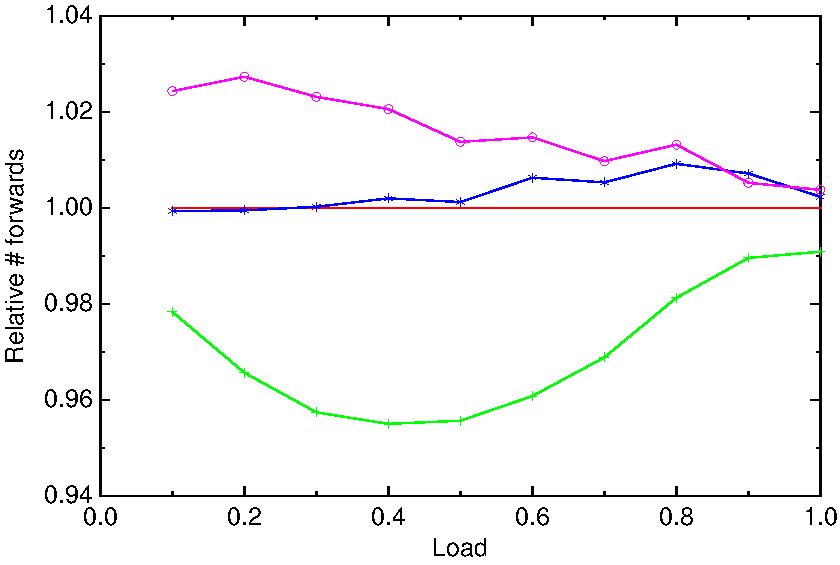
\includegraphics[width=0.9\textwidth]{../data/neighbors.pdf}
 \end{figure}
\end{frame}

\begin{frame}
\frametitle{Forward anywhere - Results}
\begin{figure}[h!tb]
 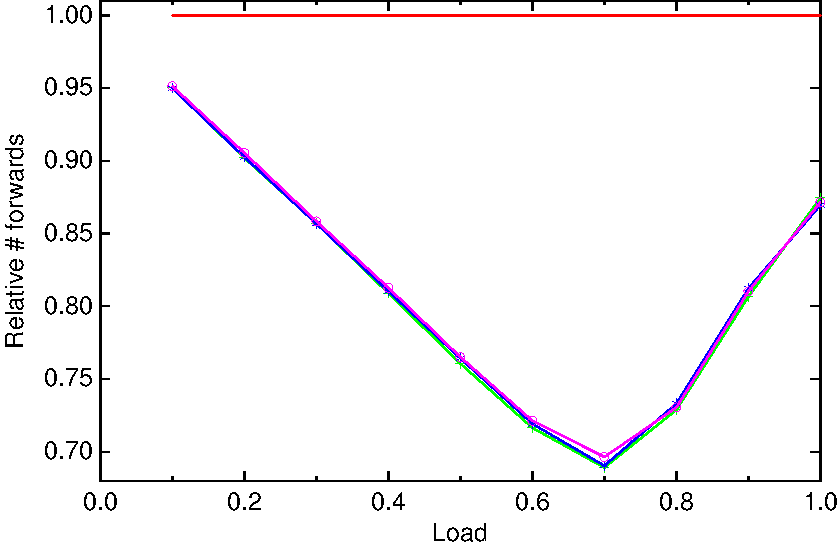
\includegraphics[width=0.9\textwidth]{../data/anywhere.pdf}
 \end{figure}
\end{frame}

\begin{frame}
\frametitle{$N$ CPUs per server}

\begin{columns}[t]
\begin{column}{0.45\textwidth}
\vspace{5em}
\begin{itemize}
 \item Divide ring size by $N$
 \item Multiply \#forwards by $N$
 \item Upper bound of the performance
\end{itemize}
\end{column}
\begin{column}{0.55\textwidth}
\begin{figure}[h!tb]
 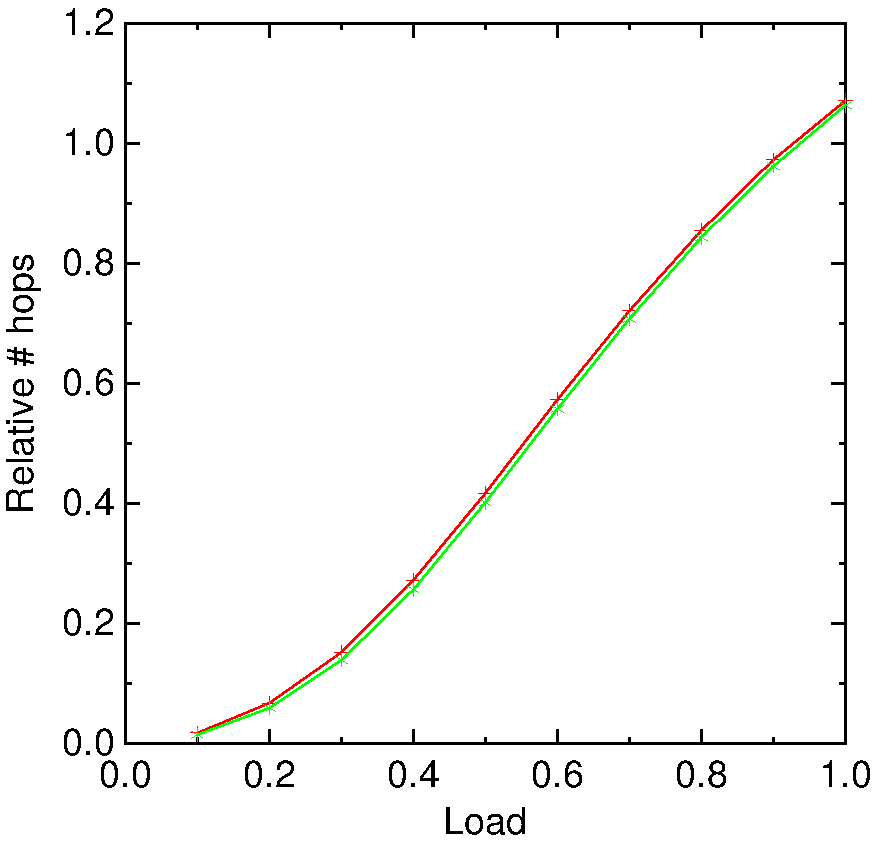
\includegraphics[width=\textwidth]{../data/right_5_2.pdf}
 \end{figure}
\end{column}
\end{columns}

\end{frame}

\section{Numerical validation}

\begin{frame}
\frametitle{Numerical validation}
\begin{itemize}
 \item Transform problem into Markov Chains
 \item Compute steady state distribution
 \item Extract the number of forwards
\end{itemize}
\end{frame}

\begin{frame}
\frametitle{Example}
\begin{center}
\hspace*{-2em}
\scalebox{0.8}{
$ \begin{blockarray}{ccccccccc}
    & 000 & 001 & 010 & 011 & 100 & 101 & 110 & 111 \\
    \begin{block}{c[cccccccc]}
    000 & -3 \lambda & \lambda & \lambda & 0 & \lambda & 0 & 0 & 0 \\
    001 & \mu & -3\lambda-\mu & 0 & (2-p)\lambda & 0 & (1+p)\lambda & 0 & 0 \\
    010 & \mu & 0 & -3\lambda-\mu & (1+p)\lambda & 0 & 0 & (2-p)\lambda & 0 \\
    011 & 0 & \mu & \mu & -3\lambda-2\mu & 0 & 0 & 0 & 3\lambda \\
    100 & \mu & 0 & 0 & 0 & -3\lambda-\mu & (2-p)\lambda & (1+p)\lambda & 0 \\
    101 & 0 & \mu & 0 & 0 & \mu & -3\lambda-2\mu & 0 & 3\lambda \\
    110 & 0 & 0 & \mu & 0 & \mu & 0 & -3\lambda-2\mu & 3\lambda \\
    111 & 0 & 0 & 0 & \mu & 0 & \mu & \mu & -3\mu \\
    \end{block}
  \end{blockarray}
$%
}
Random left/right \\ Ring size = 3
\end{center}
\end{frame}

\begin{frame}
\frametitle{Forward to neighbors}
\begin{figure}[h!tb]
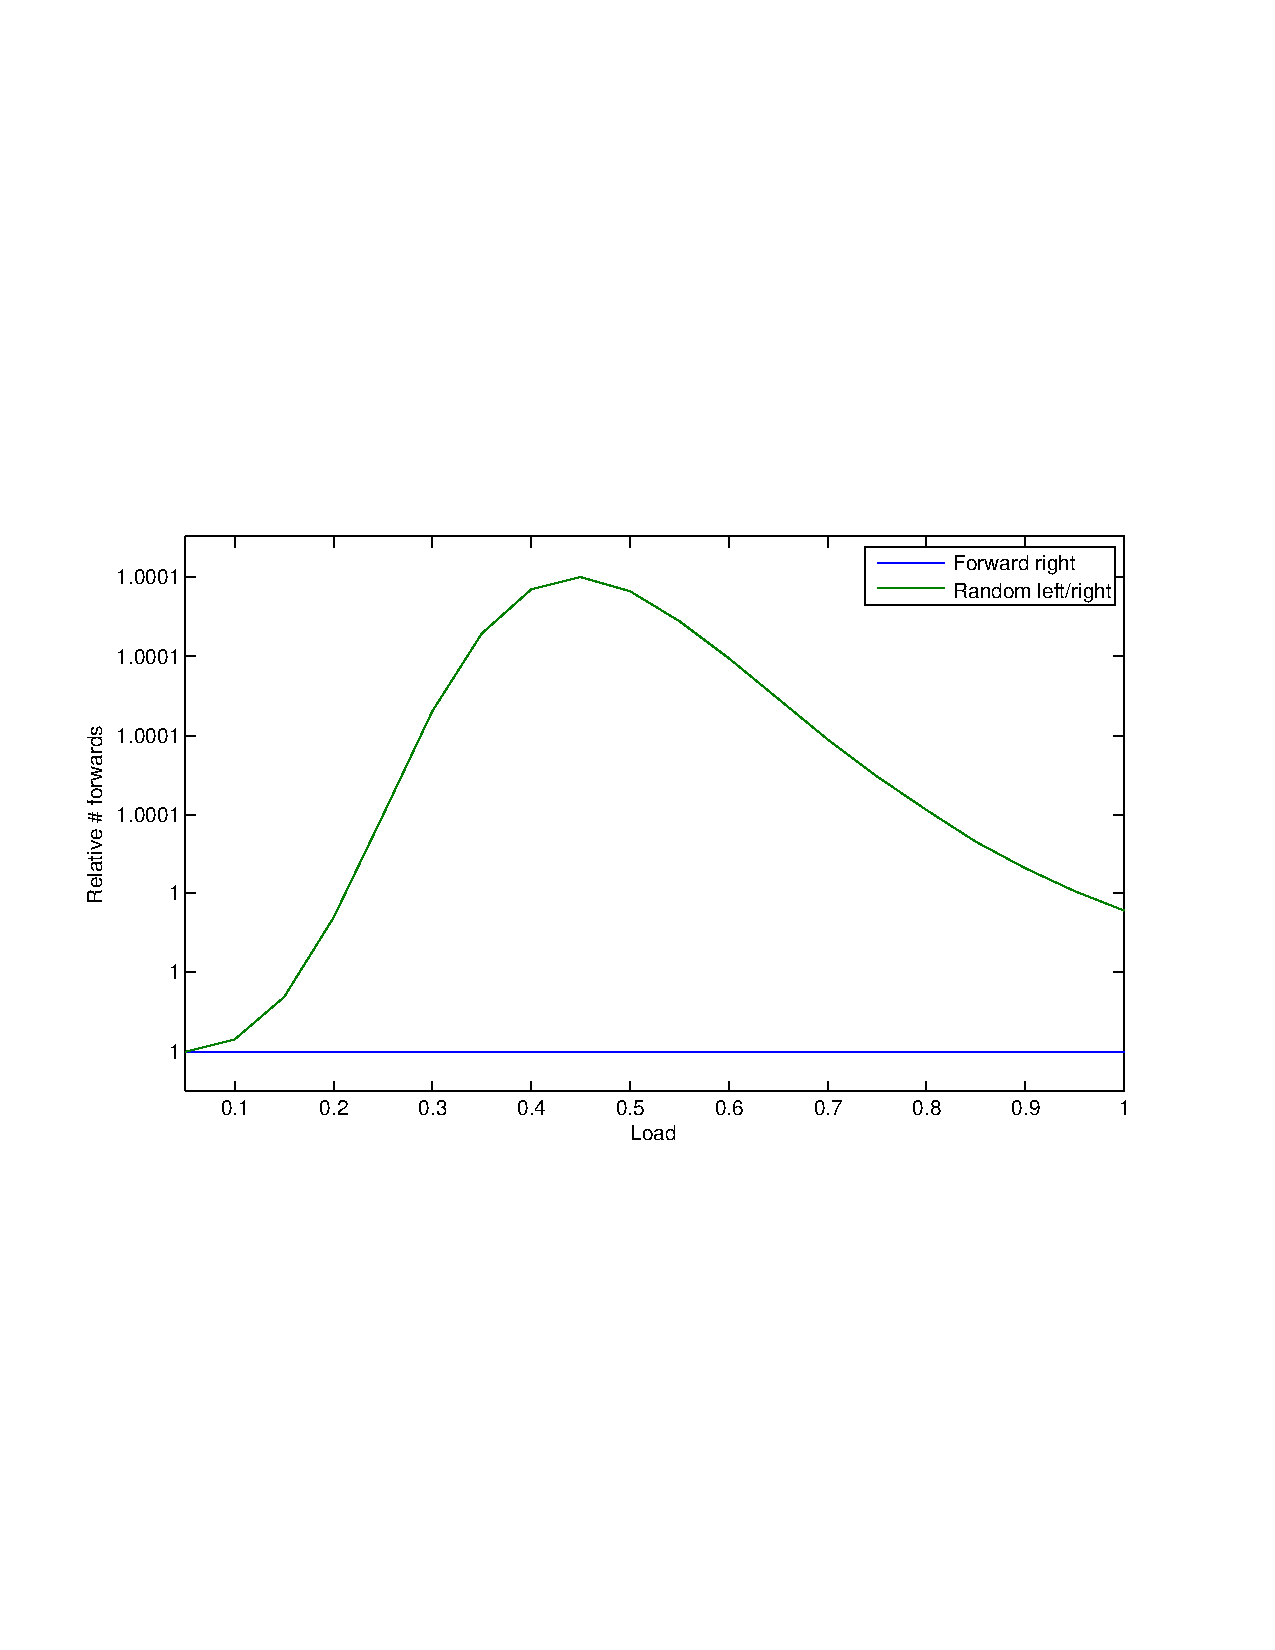
\includegraphics[width=\textwidth,clip=true,trim=4em 22em 6em 23em]{../resources/validate_rlr.pdf}
\end{figure}
\end{frame}

\begin{frame}
\frametitle{Random left/right}
\begin{figure}[h!tb]
\centering
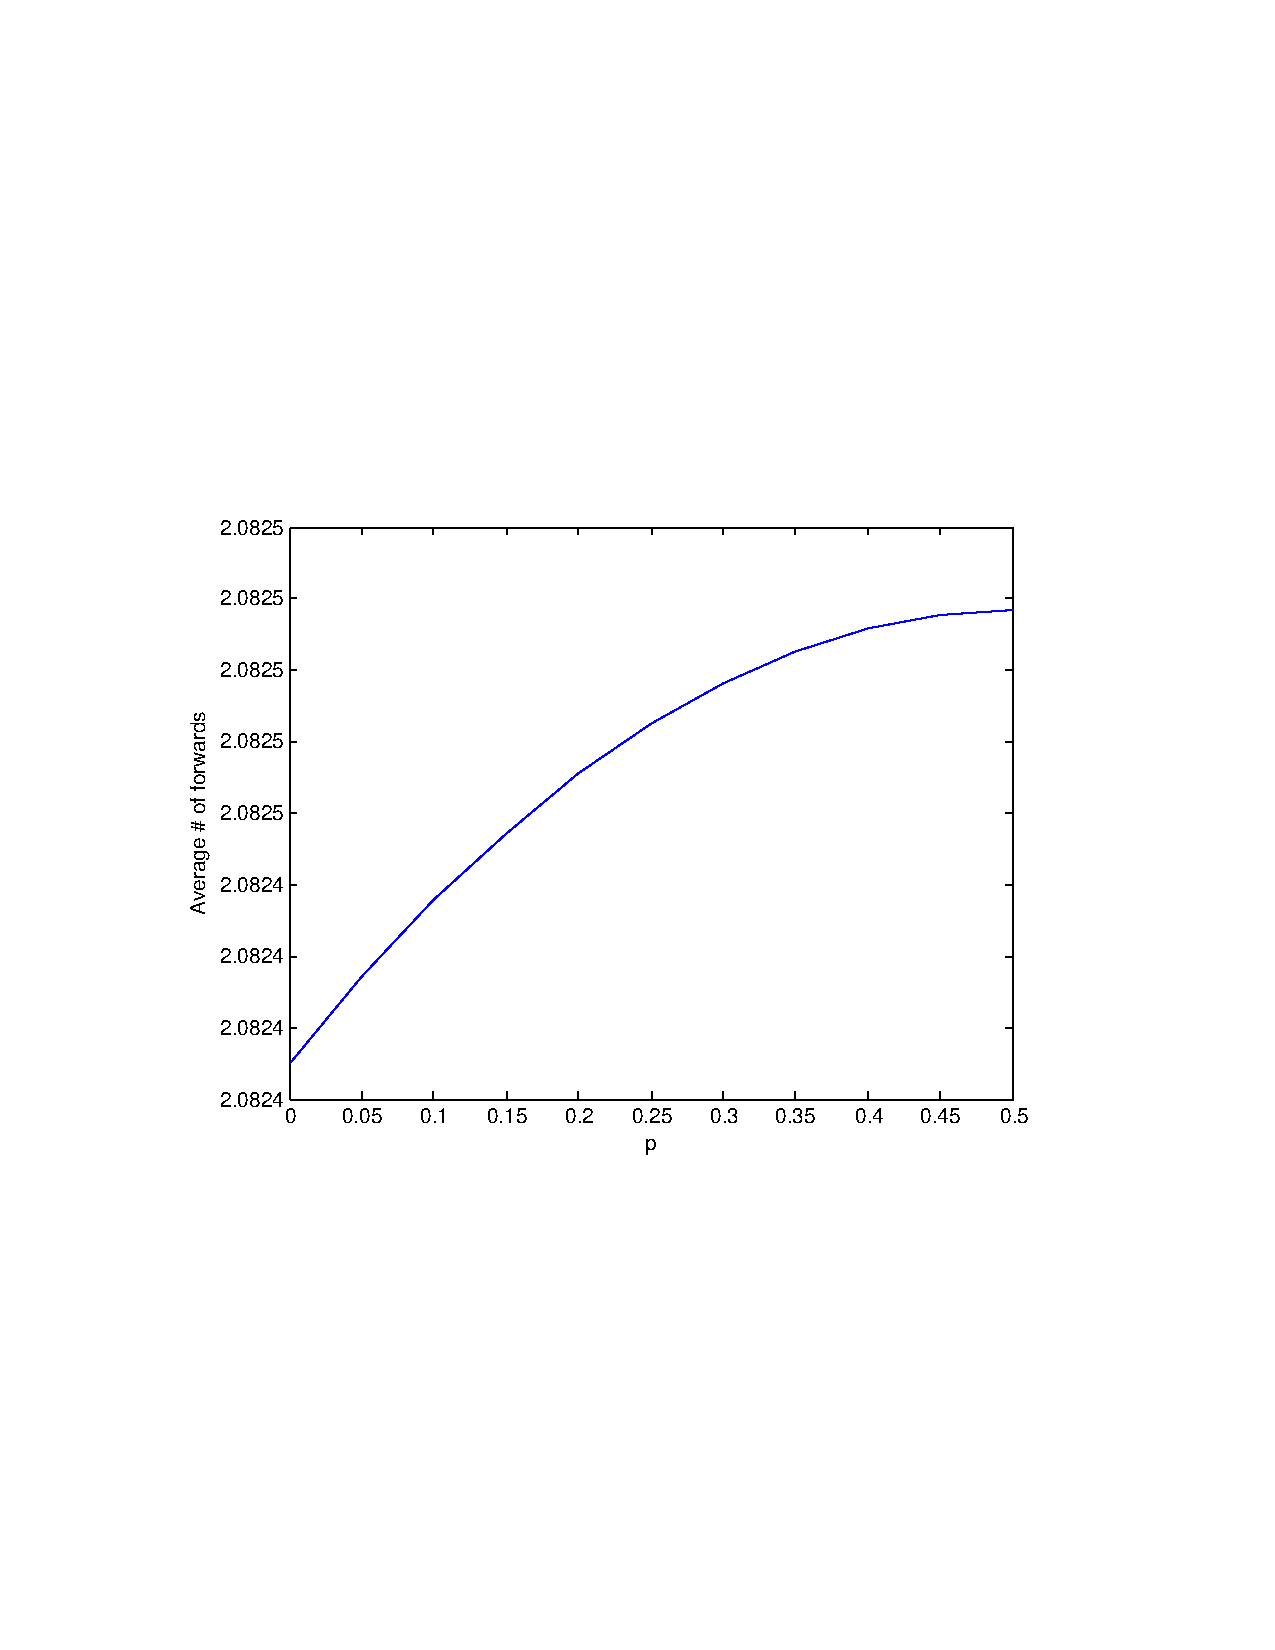
\includegraphics[clip=true, trim=8em 21em 9em 22em, width=0.8\textwidth]{../resources/plotrandlrp.pdf}
\end{figure}
\end{frame}

\begin{frame}
\frametitle{Forward anywhere}
\begin{figure}[h!tb]
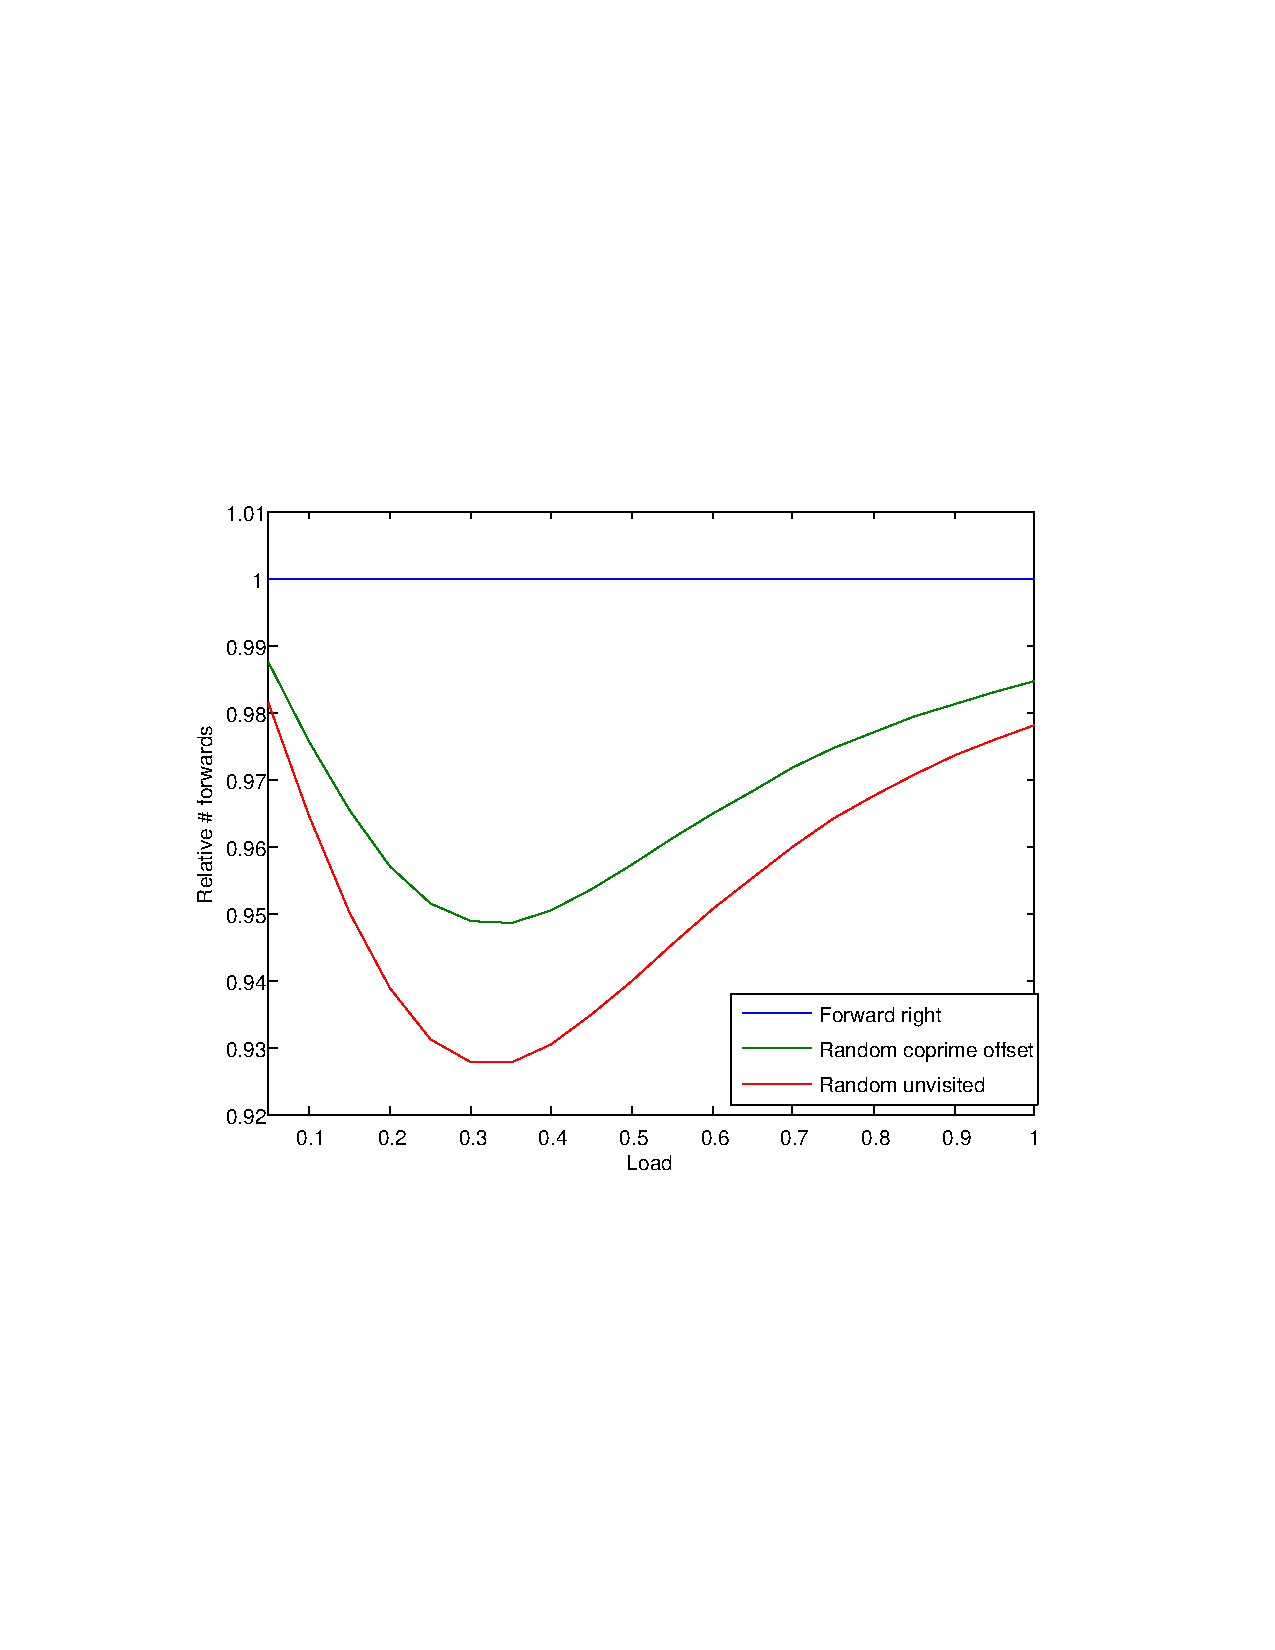
\includegraphics[width=\textwidth,clip=true,trim=4em 22em 6em 23em]{../resources/validate.pdf}
\end{figure}
\end{frame}


\begin{frame}
\frametitle{Random coprime offset}
\begin{figure}
	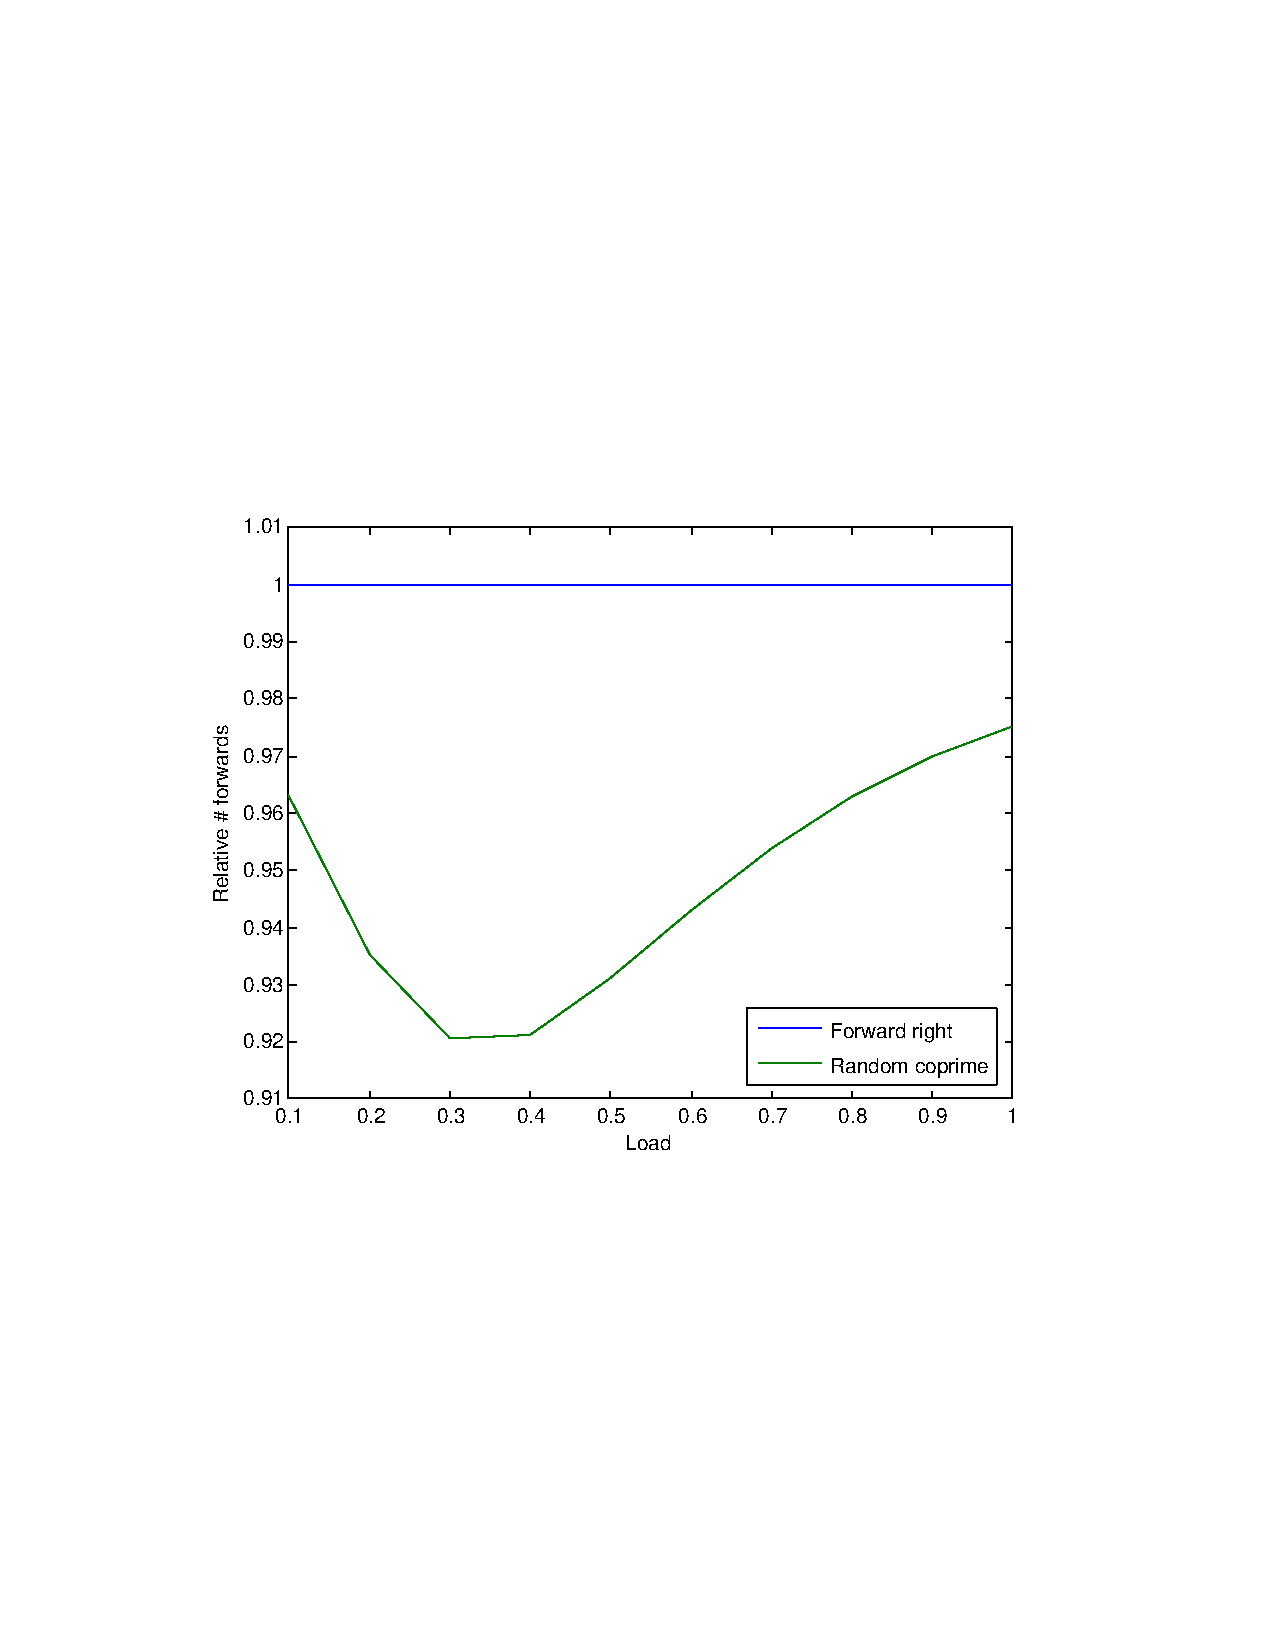
\includegraphics[clip=true, trim=9em 22em 9em 22em, width=0.5\textwidth]{../resources/plotrandcoprime11.pdf}
	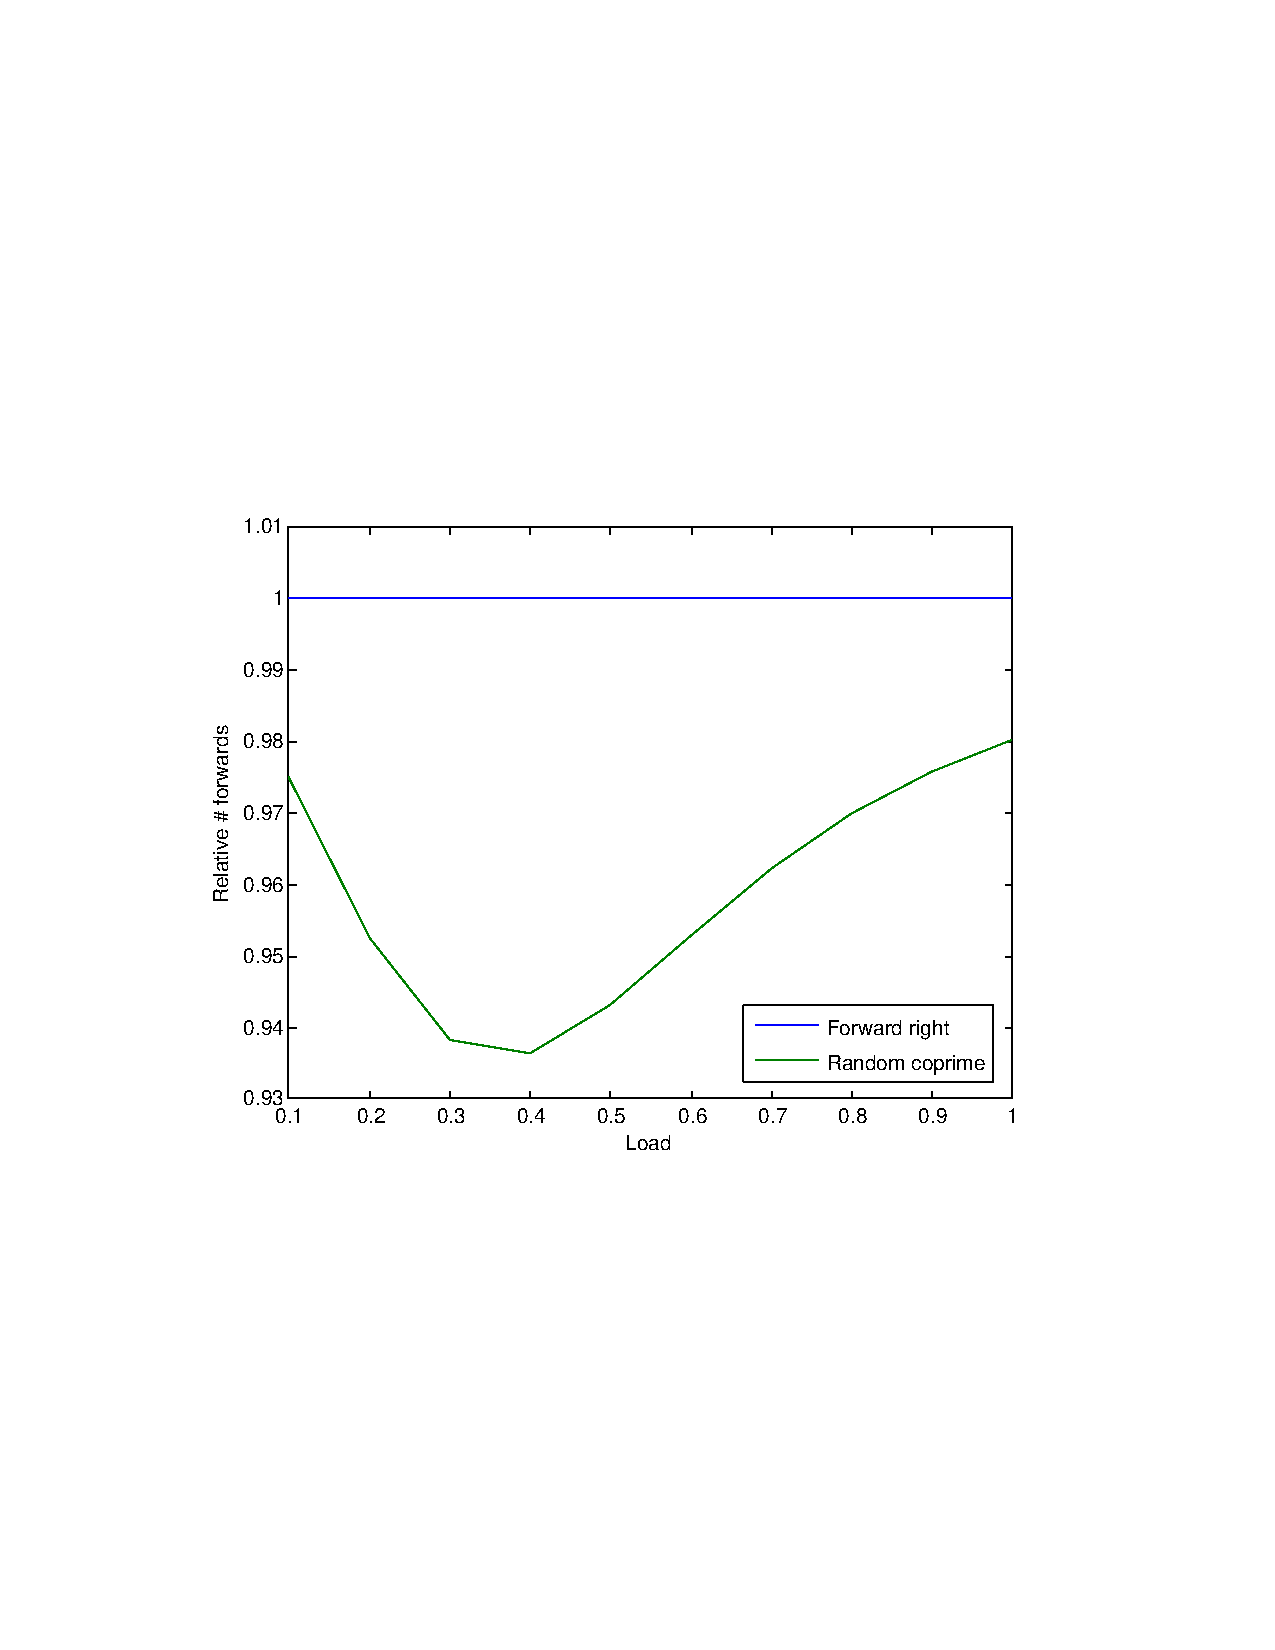
\includegraphics[clip=true, trim=9em 22em 9em 22em, width=0.5\textwidth]{../resources/plotrandcoprime12.pdf}
\end{figure}
\begin{center}
Random coprime offset for $N=11$ and $N=12$
\end{center}
\end{frame}

\begin{frame}
\frametitle{Lumping states}
\begin{itemize}
 \item Many states are redundant
 \item Compress the matrix using 1 entry per redundant state
 \item Example: 0011 = 0110 = 1100 = 1001
\end{itemize}
\vspace{2em}\[\begin{blockarray}{ccccc}
    & 000 & 001 & 011 & 111 \\
    \begin{block}{c[cccc]}
    000 & -3\lambda & 3\lambda & 0 & 0 \\
    001 & \mu & 3\lambda-\mu & 3\lambda & 0 \\
    011 & 0 & 2\mu & 3\lambda-2\mu & 3\lambda \\
    111 & 0 & 0 & 3\mu & -3\mu \\
    \end{block}
\end{blockarray}\]
\end{frame}


\begin{frame}
\frametitle{Equivalences}
\begin{itemize}
 \item Small $N$
 \item High load
 \item Random left/right vs forward right
 \item (Random) Coprime offset vs (random) left/right
 \item Random Coprime offset vs random unvisited
\end{itemize}

\end{frame}

\section{Conclusion}
\begin{frame}
\frametitle{Wrap up}
\begin{itemize}
 \item Left/right $>$ Forward right $>$ Random left/right
 \item Random unvisited $>$ (Random) Coprime offset
 \item Multiple CPUs per server
 \item Lumping Markov Chains
\end{itemize}

\end{frame}

\begin{frame}
\frametitle{Questions}
\begin{figure}[h!tb]

\includegraphics[height=0.7\textheight]{../resources/question.jpg}
\end{figure}
\end{frame}

\end{document}
